\section{Messaufbau}
In diesem Kapitel befinden sich alle Komponenten, welche für den Messaufbau benötigt wurden. Dazu gehören die Spannungsverstärkerschaltung, welcher auf dem Arduino montiert ist, das eingebaute Filter sowie der Arduino, der für die verschiedenen Funktionen programmiert wurde.
\subsection{Laboraufbau}
Um die Simulationen in die Praxis umzusetzen, wurde ein \grqq T-Drive 3Ph compact Thyristorsteller\grqq \hspace{0.03cm} von der Firma Chemtronic, vom Betreuer zur Verfügung gestellt. Wie der Name des Produktes schon sagt, arbeitet dieser Thyristorschaltung mit 3 Phasen. Für die Ansteuerung des Zündwinkels kann ein Potenziometer verwendet werden, dies hat jedoch den Nachteil, dass der Zündwinkel von Hand eingestellt werden muss. Jedoch kann für die Ansteuerung auch ein Spannungssignal von \SI{0}{V} - \SI{10}{V} benutzt werden. Dieses Spannungsignal entsprich linear dem Zündwinkel 180\textdegree \hspace{0.02cm} bis 0\textdegree \hspace{0.02cm} der Thyristoren. Um dieses Spannungssignal erzeugen zu können, wurde ein Arduino Mega 2560 verwendet. Er erzeugt jedoch nur eine Ausgangsspannung von \SI{5}{V}. Deshalb wurde eine Spannungsverstärkungsschaltung entworfen, die die Spannung verdoppelt. Die PWM-Funktion im Arduino konnte genutz werde, damit die Spannung variabel bleibt. Das PWM-Signal läuft mit einer Frequenz von \SI{490}{Hz}. 

Für die Ansteuerung des Thyristorstellers sollte zwingend eine reine DC-Spannung geliefert werden, da

Deshalb wurde zusätzlich ein Tiefpass-Filter erster Ordnung am Ausgang des Arduinos eingebaut, mit einer Cut-off Frequenz von \SI{1}{Hz}.  
\todo{nicht klar}

\subsubsection{Filter}
Um die passiven Elemente des Tiefpassfilters zu berechnen, wurde folgende Grundformel verwendet.
\begin{equation}
f = \frac{1}{2 \cdot \pi \cdot R_1 \cdot C_1}
\end{equation}


Um die Kapazität des Kondensators oder den Widerstand zu bestimmen, wurde die Kreisfrequenz auf $f$ = \SI{1}{Hz} gesetzt. Ausserdem wählte man die Kapazität auf \SI{10}{\mu F}. Dies ergab einen Widerstand von \SI{16}{\Omega}. 


%Dabei wurde $f$ = \SI{1}{Hz} eingesetzt und so kann die Kapazität oder der Widerstand frei gewählt werden. Für die Kapazität wurde \SI{10}{\mu F} ausgesucht. Somit ergab sich einen Widerstand von \SI{16}{\Omega}. Die Bauteile wurden aufgrund der vorhandenen Bauteile im Labor ausgewählt.


\subsubsection{Verstärkerschaltung}
Die Verstärkung einer nicht invertierenden Verstärkungsschaltung wird wie folgt berechnet:
\begin{equation}\label{eq:Verstärkerschaltung}
V_u = 1 + \frac{R_3}{R_2}
\end{equation}
Um die Ströme klein zu halten, wurden Widerstände von \SI{12}{k\Omega} verwendet. Die Verstärkung muss den Faktor zwei haben damit  die Spannung verdoppelt wird. Daher wurden die beiden Widerstände gleich gross gewählt.


\newpage
\begin{figure}[ht!]  
	\centering 
	\begin{minipage}[t]{.76\textwidth} \centering 
		\centering
		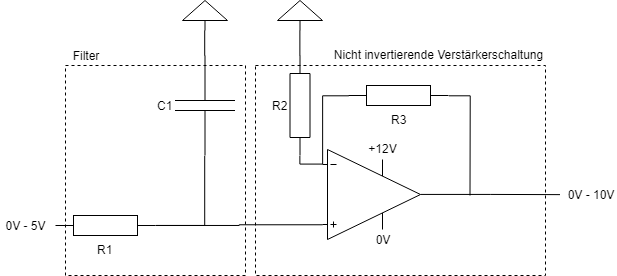
\includegraphics[scale=0.555]{Schema_Verstaerkerschaltung.png}	
		\caption{Schema Verstärkerschaltung}\label{fig:Verstaerkerschaltung}
	\end{minipage}	
	% 
	\begin{minipage}[b]{.23\textwidth}
		\centering
		\begin{tabular}{|l|l|}
			\hline
			R$_1$ & \SI{16}{k\Omega} 	\\ 	\hline
			R$_2$ & \SI{11}{k\Omega} 	\\ 	\hline
			R$_3$ & \SI{12}{k\Omega} 	\\	\hline
			C$_1$ & \SI{10}{\mu F} 		\\	\hline
		\end{tabular}
		\caption{Werte der Bauteile}
		\label{tab:Verstaerkerschaltung}
	\end{minipage}
\end{figure} 



Nach dem Aufbau der Verstärkerschaltung, wurde die Ausgangsspannung mit einem Duty Cycle von 1 gemessen. Dabei hat man den Wert von \SI{9.885}{V} erhalten. Dies bedeutet, dass der Thyristorsteller nicht voll ausgesteuert wird. Damit man die \SI{10}{V} erhält, wird bei der Verstärkerschaltung die Verstärkung erhöht. Mit der Formel \ref{eq:Verstärkerschaltung}  konnte sie neu berechnet werden:

\begin{equation}
V_u = 1 + \frac{12k\Omega}{11k\Omega} = 2.09
\end{equation}
Nach dem Einbau des neuen Widerstandes $R2$, wurde am Ausgang  eine Spannung von \SI{10.2}{V} gemessen. Somit steht der ganze Bereich von \SI{0}{V} - \SI{10}{V} zur Verfügung.

\subsection{Laboraufbau mit einem Widerstand}
Nach dem Feststellen der Funktionalität der Spannnungsverstärkungsschaltung, konnte mit dem Laboraufbau begonnen werden. Hierbei wurde ein variabler-, dreiphasiger Culatti-Widerstand als Last benutzt. Dieser hat den Vorteil das die Last bei allen Phasen symmetrisch sind. Um den Strom klein zu halten, wurde ein Widerstand von \SI{150}{\Omega} gewählt. Der Aufbau der Messschaltung ist auf der Abbildung \ref{fig:Messaufbau} ersichtlich.


\begin{figure}[ht!]
	\centering
	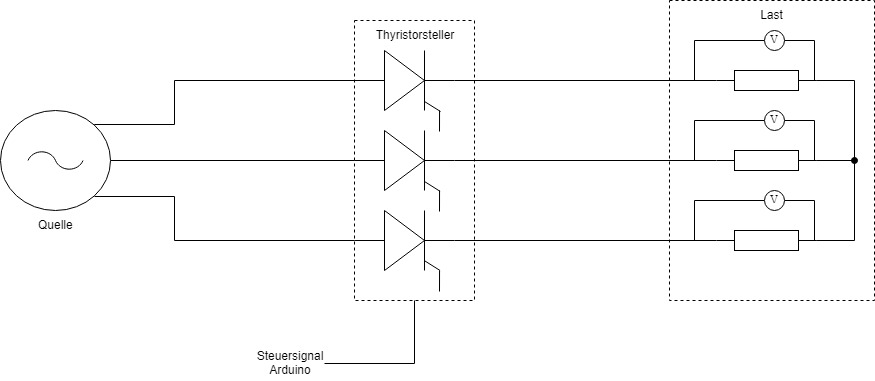
\includegraphics[width=\textwidth]{Messaufbau.png}	
	\caption{Schema Laboraufbau mit einem dreiphasigen Widerstand in Stern geschaltet}\label{fig:Messaufbau}
\end{figure}

Die Last wurde zudem noch in Dreieck geschaltet, um einen Unterschied von den Strömen und den Spannungen zur Sternschaltung zu erhalten.

\subsection{Laboraufbau mit einer ASM}

Gleich wie beim Laboraufbau des Widerstands wurde bei diesem Versuchen ein Asynchronmotor als Last in den Stromkreis eingebaut. Dabei wurde er in Stern und in Dreieck geschaltet. Ein Vorteil des Motors, der Marke Lukas Nülle mit einer Leistung von \SI{0.3}{kW} ist, dass ein integrierter Drehzahlgeber vorhanden ist, um die Drehzahl zu messen. Die Maschine verhält sich nicht wie der Culatti rein ohmsch, sonder ohmschi-induktiv da verschiedene Reaktanzen in der Erreger- und Ankerwicklung vorkommen. Daher werden die Spannungen und die Ströme der Maschine anders aussehen als beim Widerstand. Ein weiterer interessanter Punkt ist, dass beim Wegschalten der Spannung, der Motor weiter dreht und so träge auf Veränderungen reagiert.  


%Für die ASM wurde eine Maschine der Marke Lukas Nülle mit einer Leistung von \SI{0.3}{kW} verwendet. Dies hat den Grund, dass bei dieser Maschine ein Drehzahlgeber vorhanden war um die Drehzahlen messen zu können. Da die Maschine nicht wie der Widerstand, eine rein ohmsche Last ist, verhielten sich die Spannungen und Ströme anders. Ein weiterer interessanter Punkt bei dem Motor ist, dass wenn die Spannung abgeschaltet wird, die Motor sich noch ausdrehen muss und so sehr träge auf Veränderungen reagiert.

\subsection{Arduino}

Das Arduino-Programm, welches den Thyristorsteller ansteuert, wurde mit der Arduinosoftware geschrieben. Ein Vorteil des Arduinos ist, dass die Software öffentlich zugänglich ist. Ausserdem sind einige nützliche Beispielcodes im Internet vorhanden. Mit den verschiedenen I/O Pins können Spannungen bis zu \SI{5}{V} gemessen und ausgegeben werden.
 

\subsubsection{Phasenanschnittssteuerung mit Arduino}
Die Phasenanschnittsteuerung wird mit der einfachen \SI{0}{V} bis \SI{10}{V} Ansteuerung des Thyristorstellers realisiert. Dabei ist die Ansteuerungskennlinie linear und so entsprechen \SI{10}{V} einem Zündwinkel von 0\textdegree und \SI{0}{V} einem Zündwinkel von 180\textdegree . Diese Ansteuerungsbereich muss auf die 0 bis 255 Werte umgerechnet werden, da der analogWritbe()-Bereich des Arduinos so konzipiert ist. Wenn zum Beispiel ein Winkel von 90\textdegree \hspace{0.02cm} erwünscht ist, muss ein Wert von 127 ausgegeben werden.

\subsubsection{Schwingungspaketsteuerung mit Arduino}
Die Schwingungspaketsteuerung funktioniert mit dem Thyristorsteller nicht so einfach, da dieser nur für den Phasenanschnitt konzipiert ist. Jedoch kann beim Arduino zwischen HIGH und LOW mit einer bestimmten Zeitverzögerung dazwischen, umgeschaltet werden. Das Problem welches dabei auftritt ist, dass der Thyristorsteller und die Spannungsverstärkerschaltung zusammen eine Zeitverzögerung von \SI{0.2}{s} haben. So schaltet der Sinus verzögert ein und daraus folgt ein sanftes Hochfahren von \SI{0.35}{s}. Ein hartes Zu- und Wegschalten wie in den Simulationen gezeigt, ist deshalb nicht möglich.


\subsubsection{Hartes Auf- und Absteuern}
Um das harte Auf- und Absteuern zu implementieren, wurden die beiden vorherigen Verfahren miteinander kombiniert. Anstatt jedoch nur einen Winkel vorzugeben, wurde mit einer for-Schleife die Ansteuerungsspannung und somit der Zündwinkel linear erhöht. Sobald sich die Spannung auf dem Maximum befindet, wartet der Thyristorsteller für \SI{0.2}{s}. Eine gewisse Zeit wird die maximale Spannung ausgegeben. Danach wird mit einer zweiten for-Schleife Heruntergefahren. Wenn die minimale Spannung erreicht ist, wartet das Programm\SI{0.1}{s} bis das nächste Hochfahren beginnt. Dies hat den Grund, da sonst das Spannungssignal nicht auf Null geht. Die zwei for-Schleifen befindet sich in einer dritten for-Schleife, die die Schwingungspaketsteuerung simuliert. Mit ihr kann eingestellt werden, wie oft das Hoch- und Runterfahren durchgeführt wird. Wenn zum Beispiel fünf von zehn Pakete angesteuert werden, fährt das Programm fünf mal Hoch- und Runter und sperrt die restlichen fünf Pakete. 

\subsubsection{Sanftes Auf- und Absteuern}
Bei dem sanften Auf- und Absteuern ist die Steigung des Hoch- und Runterfahren flacher als die bei dem harten Auf- und Absteuern. Zusätzlich wird nach dem Erreichen der maximalen Spannung eine Verzögerung von \SI{6}{s} eingebaut. Damit das Signal \SI{6}{s} auf dem Maximum bleibt. Anschliessend fährt das Programm die Spannung mit der gleichen Steigung wie beim Hochfahren runter und bleibt für \SI{3}{s} auf \SI{0}{V}. Dies kann beliebig oft wiederholt werden.


\subsubsection{Drehzahlmessung für eine Reglerauslegung}
Um die Drehzahl der Asynchronmotors zu messen und regeln zu können, wurde eine Drehzahlregelung im Arduino programmiert. Dabei wird die Spannung über dem Drehzahlgeber des Asynchronmotors benötigt. Sie beträgt bei der maximalen Drehzahl von \SI{2800}{U/min}, \SI{58.8}{V}. Die Spannung ist linear von der Drehzahl abhängig und beträgt so, bei zum Beispiel \SI{1400}{U/min}, \SI{29.4}{V}. Da der Arduino nur eine maximale Spannung von \SI{5}{V} einlesen kann, wird mit Hilfe eines Spannungsteiler die Spannung des Drehzahlgebers linear reduziert. Mit folgender Grundformel des Spannungsteilers und des freien wählen eines Widerstand $R1$, konnte daraus $R2$ bestimmt werden:

\begin{equation}
U_2=U_{Ges} \cdot\frac{R1}{R1 + R2} \Longrightarrow 4.94 V = 58.8 V \cdot \frac{56k\Omega}{56k\Omega + R2}
\end{equation}

Das Resultat des Widerstand ist \SI{611}{k\Omega} und somit konnte die Spannung mit dem Arduino gemessen werden. Mit dem ADC wird sie in 1024 verschieden Werte aufgeteilt. Der Wert 512 entspricht so einer Spannung von \SI{2.5}{V}.\todo{Einfügen Quelle für Spannungsmessung} Danach wird dieser Wert mit den Widerstandswerten des Spannungsteiler auf die Originalspannung zurück gerechnet. Bei dem Regler wird für den Sollwert ein gewünschter Spannungswert vorgegeben. Anschliessend wird der Istwert vom Sollwert abgezogen, dadurch erhält man die Differenz. Da der Ausgabewert des Arduinos einem Wert zwischen 0 bis 255 entspricht, muss die Differenz umgerechnet werden. Zusätzlich wird ein PI-Regler benötigt, damit eine exakte und schnelle Regelung möglich ist.
Mit der Formel \ref{eq:digitaler_PI_Regler} wird die Ausgangsspannung eines digitaler PI-Regler berechnet: \cite{Quelle_Marco} 
\begin{equation}\label{eq:digitaler_PI_Regler}
Y(k) = Y(k-1)+ B_0U(k)+B_1U(k-1)
\end{equation}
Wobei $Y$ die Ausgangsspannung, $U$ die Differenzspannung und $k$ der Laufparameter sind \cite{PI_Regler}. Die Parameter $B_0$ und $B_1$ werden folgendermassen berechnet:
\begin{equation}\label{eq:B0}
B_0 = \left(K_p + \frac{K_iT}{2}\right) 
\end{equation}
\begin{equation}\label{eq:B1}
B_1 = -\left(K_p - \frac{K_iT}{2}\right) 
\end{equation}

Danach muss die Spannungsdifferenz von der Ausgangsspannung subtrahiert werden. Das Resultat der Berechnung wird in die 0 bis 255 Werte umgerechnet und mit dem analogWrite() ausgegeben. Die Werte der Ausgangsspannung und der Differenzspannung werden nach der Ausgabe in den Laufparameter $k-1$ geladen. Das Problem mit dem PI-Regler ist, dass der Thyristorsteller und die Spannungsverstärkung eine Totzeit besitzen. Ausserdem hat der Aurduino keine konstate Abtastrate bei dieser Anwendung. Dadurch ist das Auslegen eines guten Reglers nicht möglich. Der Code für die Drehzahlregelung befindet sich im Anhang. \todo{Kapitel angeben}

\begin{figure}[ht!]
	\centering
	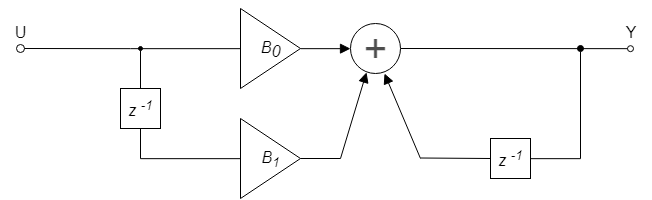
\includegraphics[width=\textwidth]{BlockdiagrammPI.png}	
	\caption{Blockdiagramm eines digitalen PI-Reglers}\label{fig:PIRegler}\cite{PI_Regler}
\end{figure}







